\chapter{Introduction}

\section{Définitions. Rappels}

Dans ce cours, on va s’intéresser à des méthodes numériques pour calculer, ou approcher, la solution des problèmes tels que :

\begin{itemize}
\item La résolution de grands systèmes linéaires $Ax = b$, où $A$ est une matrice réelle carrée.
\item La détermination de valeurs propres de la matrice $A$.
\item La résolution d’équations non linéaires $f(x) = 0$.
\item Le calcul d’une solution d’une équation différentielle ordinaire ou équation aux dérivées partielles.
\end{itemize}

On supposera en général que la solution existe ; le but est de trouver des méthodes rapides et précises pour déterminer la ou les solutions. Dans la résolution numérique d’un problème, il est essentiel de tenir compte des notions présentées dans la suite.

\subsection{Instabilité du problème}
Certains problèmes mathématiques sont \textbf{instables} : de petites perturbations des paramètres, dont dépend le problème, vont engendrer de grandes variations des solutions. Des exemples sont la détermination des racines d’un polynôme, la résolution de l’équation de la chaleur inversée, ou certains systèmes dynamiques (modèle de Lorenz en météorologie).

Comme dans les applications les paramètres des modèles mathématiques viennent souvent d’expériences (donc avec une certaine imprécision), on utilise de préférence des modèles stables.

Soit $s = A(e)$ un algorithme ou problème qui, en fonction du paramètre $e$ en entrée, produit le résultat $s$. On s’intéresse à la stabilité de $A$ par rapport à une perturbation $\delta e$ de l’entrée. Pour cela, on veut majorer l’erreur relative en sortie, grâce à l’erreur relative en entrée. Si l’on peut écrire :

$$
\frac{|\tilde{s} - s|}{|s|} = \frac{|A(e + \delta e) - A(e)|}{|A(e)|} \leq c(A) \frac{|\delta e|}{|e|}
$$

où la constante $c(A)$ est la meilleure borne possible pour obtenir cette inégalité, alors on appelle $c(A)$ le \textbf{conditionnement} du problème $A$.

\subsection{ Erreurs d’approximation}
Ce type d’erreur apparaît lorsque l’on remplace un problème continu par un problème discret. On est obligé de remplacer un objet mathématique, souvent défini grâce à des limites, par un nombre fini d’opérations numériques ; on parle dans ce contexte aussi d’\textbf{erreur de troncature}. Quand le pas de discrétisation tend vers zéro (c’est-à-dire le nombre d’opérations tend vers l’infini), la formulation discrète doit tendre vers la formulation continue du problème.

Les formules de quadrature pour calculer des intégrales sont des exemples de formulations discrètes. La méthode des trapèzes pour le calcul numérique de l’intégrale d’une fonction $f$ sur $[a, b]$ s’écrit :

$$
\int_{a}^{b} f(t)dt \approx \sum_{i=0}^{N-1} (x_{i+1} - x_i) \frac{f(x_i) + f(x_{i+1})}{2}
$$

Pour la partition $a = x_0 < x_1 < \dots < x_N = b$, le pas de discrétisation est $h = \max_{0 \leq i \leq N-1} (x_{i+1} - x_i)$, qui doit tendre vers $0$ quand $N$ tend vers l’infini.

\begin{figure}[h!]
\centering
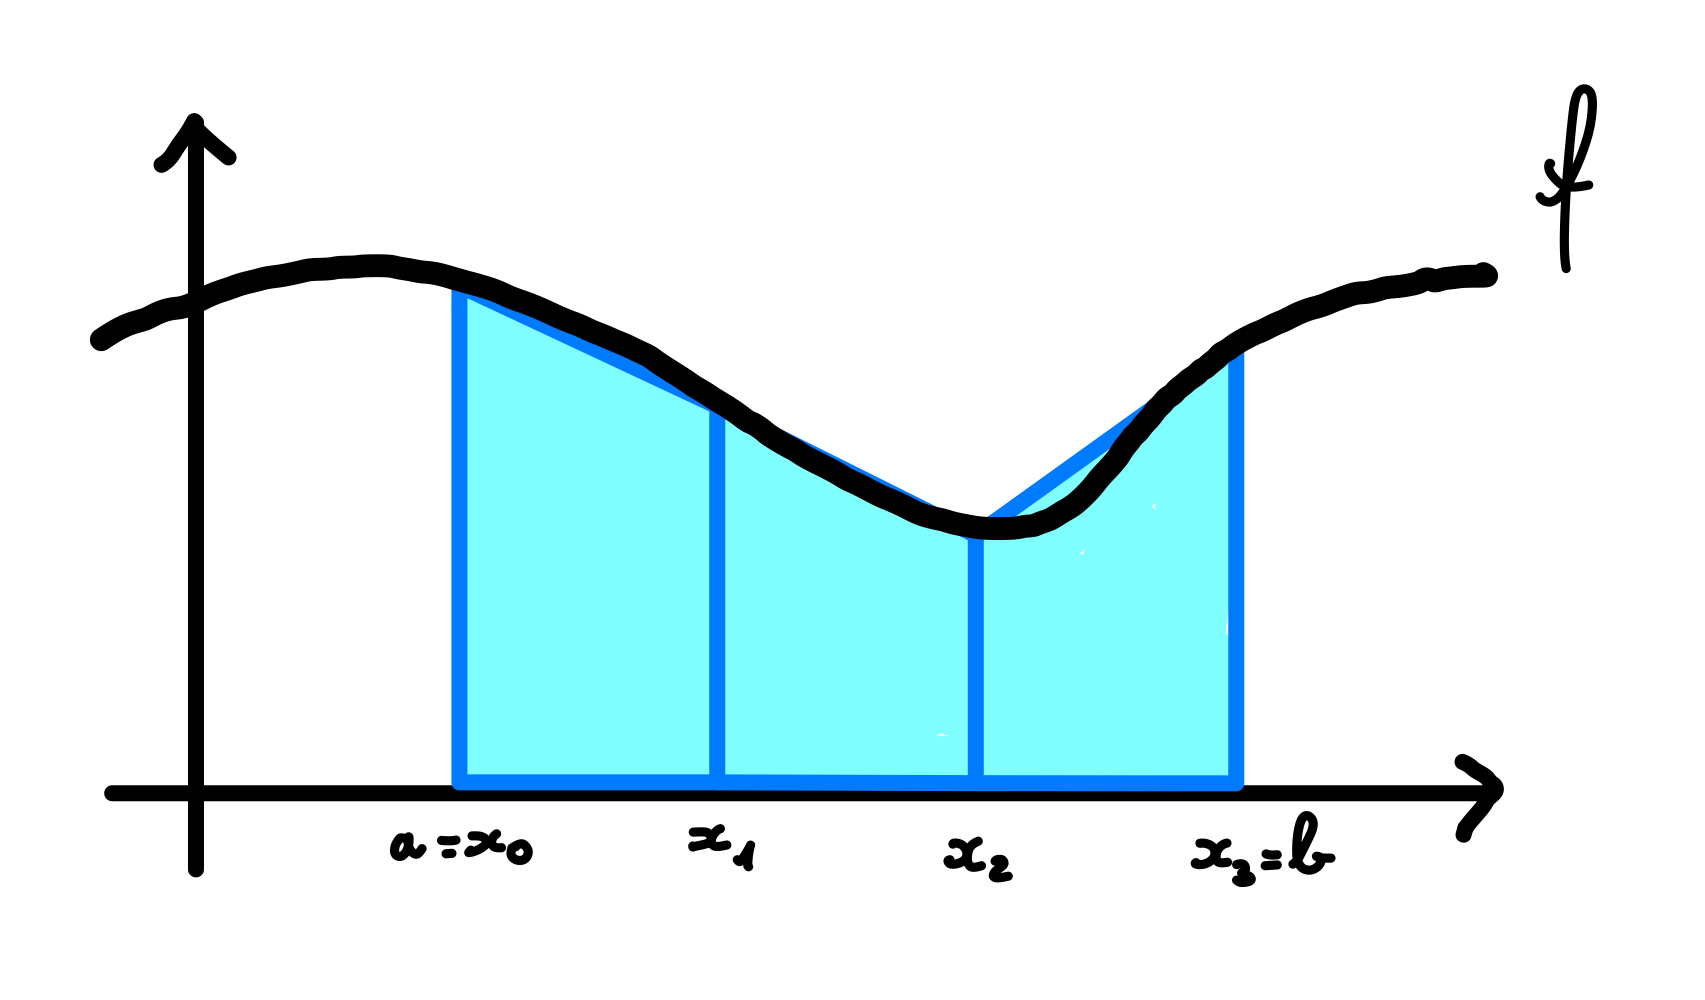
\includegraphics[width=0.45\textwidth]{CM1/Image/Courbe.jpg}
\caption{Méthode du trapèze avec $N = 3$.}
\end{figure}

D’autres exemples sont les schémas aux différences finies pour la résolution d’équations différentielles ordinaires et d’équations aux dérivées partielles qui seront abordés plus tard.

\subsection{ Erreurs d’arrondi}
Les calculs numériques sur ordinateur se font avec une précision finie. La mémoire disponible étant finie, on ne peut pas représenter les nombres réels qui ont un développement décimal infini. On peut représenter $1/3$, mais pas son écriture décimale, et on ne pourra représenter $\pi$ que par un nombre fini de décimales.

Une représentation fréquente des nombres réels est celle en \textbf{virgule flottante normalisée} :

$$
f = (-1)^s 0, d_{-1}d_{-2} \dots d_{-r} \times b^j
$$

avec $m \leq j \leq M$ et $0 \leq d_{-i} \leq b - 1$, où :
\begin{itemize}
\item $s \in \{0, 1\}$ est le signe.
\item $d_{-1}d_{-2} \dots d_{-r}$ est la mantisse ou significande.
\item $b$ est la base.
\item $r$ est le nombre de chiffres significatifs.
\end{itemize}

La précision machine pour un flottant de $r$ chiffres significatifs est $b^{1-r}$ ; c’est la distance entre $1$ et le nombre flottant immédiatement plus grand $1 + b^{1-r}$. Comme seulement un nombre fini de réels est représenté, le résultat des opérations arithmétiques de base ($+, -, \times, /$) sur ces réels n’est pas nécessairement représentable, on est obligé d’arrondir.

\textbf{L’arithmétique IEEE}, utilisée sur les machines sous Unix et Linux, définit des nombres flottants en base $b = 2$ :

\begin{itemize}
\item \textbf{Simple précision (32 bits, type float en C) :} 1 bit pour $s$, 1 octet pour l’exposant (signé) $j$ (i.e. $j \in \{-127, \dots, +128\}$), et 23 bits pour la mantisse.

Si l’on suppose que la représentation est normalisée (i.e. $d_{-1} \neq 0$), on gagne un bit significatif en utilisant la technique du bit caché et un flottant en simple précision s’écrit :

$$
f = (-1)^s 1, d_{-1}d_{-2} \dots d_{-r} \times 2^j = (-1)^s 0, 1d_{-1}d_{-2} \dots d_{-r} \times 2^{j+1}
$$

La précision machine est alors $2^{-23}$, c.-à-d. approximativement $10^{-7}$, et les flottants normalisés positifs vont de $10^{-38}$ à $10^{+38}$.

Les modules arithmétiques envoient aussi des messages qui indiquent la nature du résultat de l’opération :
\item \textbf{NaN (Not A Number) :} résultat de "$\infty - \infty$", "$\sqrt{-1}$" ou "$0/0$".
\item \textbf{+/-INF :} si le résultat est un nombre trop grand pour être représenté.
\end{itemize}

Dans Octave aussi, les nombres réels sont représentés en virgule flottante en base 2, avec $r = 53$. La précision machine est stockée dans la constante `eps` et vaut $2^{-52} \sim 2.22 \times 10^{-16}$.


\subsection{Complexité des calculs}
Pour pouvoir appliquer une méthode, il faut obtenir un résultat en un temps raisonnable. Il est donc important de pouvoir estimer le temps que l’algorithme va utiliser pour résoudre le problème. Pour cela, on compte le nombre d’opérations flottantes (angl. flops) en fonction de la taille du problème.

Souvent il suffit d’avoir un ordre de grandeur. Si $N$ est la taille du problème (p.ex. le nombre d’inconnues), on peut avoir des algorithmes en $O(N)$, $O(N \ln N)$, $O(N^2)$, $O(N^3)$, $O(N!)$, etc.

Des formules mathématiques équivalentes peuvent avoir des temps de calcul très différents en pratique, comme le montre l’exemple suivant.

\subsection{ Exemple : Coût de multiplication de matrices}
Soient $A$, $B$ et $C$ des matrices rectangulaires, de dimensions respectives $(n, m)$, $(m, p)$ et $(p, q)$. Combien d’opérations sont nécessaires pour calculer $ABC$ ?

Comme $ABC = (AB)C = A(BC)$, on a deux possibilités d’évaluation :

\begin{enumerate}
\item Le calcul de $(AB)C$ nécessite de l’ordre de $O(2np(m +q))$ opérations.
\item Le calcul de $A(BC)$ se fait en $O(2mq(n + p))$ opérations.
\end{enumerate}

Si l’on prend par exemple $n = p = 10$ et $m = q = 100$, on trouve $4 \cdot 10^4$ et $4 \cdot 10^5$. La multiplication des matrices rectangulaires étant distributive, on obtient deux fois le même résultat (aux erreurs d'arrondi près), mais le nombre d’opérations nécessaires peut varier de façon importante.

Si $n = m = p$, alors $A$ et $B$ sont des matrices carrées et le coût de leur multiplication est $O(n^3)$.

\subsection{ Ordre d’une méthode itérative}

Mis à part le nombre d’opérations total à exécuter, il peut être intéressant de comparer des vitesses de convergence.

Soit $(x^{(n)})_{n \in \mathbb{N}}$ une suite convergeant vers $x^*$. On dit que la convergence est d’\textbf{ordre} $\lambda \geq 1$, s’il existe une constante $C \in \mathbb{R}^*_+$ telle que, pour $n$ suffisamment grand :

$$
\frac{\|x^{(n+1)} - x^*\|}{\|x^{(n)} - x^*\|^\lambda} \leq C
$$

\begin{itemize}
\item Si $\lambda = 1$, il faut $C \in ]0, 1[$ pour avoir convergence et on a alors \textbf{convergence linéaire}.
\item Si $\lambda = 2$, on a \textbf{convergence quadratique}.
\end{itemize}

La quantité $(-\log_{10} \|x^{(n)} - x^*\|)$ mesure le nombre de décimales exactes derrière la virgule, la quantité $(-\log_{10} (\|x^{(n)} - x^*\| / \|x^*\|))$ indique le nombre de chiffres exacts en tout.

Pour une méthode d’\textbf{ordre 1}, on a :

$$
(-\log_{10} \|x^{(n+1)} - x^*\|) \geq (-\log_{10} \|x^{(n)} - x^*\|) - \log_{10}(C)
$$

On gagne à chaque itération $\log_{10}(1/C)$ décimales.

Pour une méthode d’\textbf{ordre} $\lambda > 1$, on a :

$$
(-\log_{10} \|x^{(n+1)} - x^*\|) \geq \lambda (-\log_{10} \|x^{(n)} - x^*\|) - \log_{10}(C)
$$

Alors $x^{(n+1)}$ a $\lambda$ fois plus de décimales exactes que $x^{(n)}$. Ainsi une méthode quadratique ($\lambda = 2$) double le nombre de chiffres exacts à chaque itération.

\section{ Utilisation d’un logiciel de calcul scientifique}

Les logiciels de calcul scientifique numérique tels que Octave, Matlab©, Scilab... font appel à des fonctions « bas niveau » en langage C ou Fortran et rassemblées dans des librairies telles que LAPACK, CLAPACK, ScaLAPACK, BLAS...

Ces codes sont programmés de façon à être aussi efficaces que possible en termes de précision, stabilité et vitesse d’exécution. En utilisant ces logiciels dans la résolution numérique d’un problème, il faut toujours garder en mémoire les problèmes cités dans la section précédente.

Dans Python, on sera amené à charger les librairies `numpy` et/ou `scipy` pour les calculs numériques et par exemple `matplotlib.pyplot` pour les graphiques.